% part I
% \titleformat{\chapter}
%   {\chap}{\thechapter}{1em}{}
% \titlespacing*{\chapter}{0pt}{3.5ex plus 1ex minus .2ex}{2.3ex plus .2ex}
%
\part{毕业论文(设计)}

\chapter{绪论(章的标题,三号仿宋加黑)}

{\bfxs{正文中文加粗}}

\begin{equation}
\frac{a}{b}
\end{equation}

\section{节的标题(小三号仿宋加黑)}

\subsection{节的标题(四号仿宋加黑)}

\subsubsection{节的标题,仿宋四号加黑}
%测试\cite{small},\textcite{small},\parencite{small}

测试\upcite{small} only available for numbib option
\chapter{正文}

\begin{figure}[H]
    \centering
    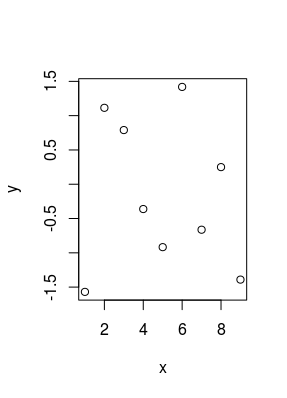
\includegraphics{../assets/sample.png}
    \caption{正态随机数}
\end{figure}

\section{节的标题(仿宋小三号加黑)}
\begin{equation}
\frac{1}{2}
\end{equation}
\chapter{test space}
\section{test space}
\subsection{test space}
\subsection{节的标题(仿宋四号加黑)}
符号说明
{\wuhao
\begin{longtable}{p{5cm}p{5cm}}
\caption{符号说明}\\
\hline
项目内容 & 特点\\
\hline
模拟& 同方差\\
\hline
\end{longtable}
}
项目内容

定理环境

\begin{theorem}
$a > b$ 且 $b > c$
\end{theorem}

\begin{corollary}
$a > c$
\end{corollary}


\begin{algorithm}
\DontPrintSemicolon
\KwData{$G=(X,U)$ such that $G^{tc}$ is an order.}
\KwResult{$G’=(X,V)$ with $V\subseteq U$ such that $G’^{tc}$ is an
interval order.}
\Begin{
$V \longleftarrow U$\;
$S \longleftarrow \emptyset$\;
\For{$x\in X$}{
$NbSuccInS(x) \longleftarrow 0$\;
$NbPredInMin(x) \longleftarrow 0$\;
$NbPredNotInMin(x) \longleftarrow |ImPred(x)|$\;
}
\For{$x \in X$}{
\If{$NbPredInMin(x) = 0$ {\bf and} $NbPredNotInMin(x) = 0$}{
$AppendToMin(x)$}
}
\nl\While{$S \neq \emptyset$}{\label{InRes1}
\nlset{REM} remove $x$ from the list of $T$ of maximal index\;\label{InResR}
\lnl{InRes2}\While{$|S \cap ImSucc(x)| \neq |S|$}{
\For{$ y \in S-ImSucc(x)$}{
\{ remove from $V$ all the arcs $zy$ : \}\;
\For{$z \in ImPred(y) \cap Min$}{
remove the arc $zy$ from $V$\;
$NbSuccInS(z) \longleftarrow NbSuccInS(z) - 1$\;
move $z$ in $T$ to the list preceding its present list\;
\{i.e. If $z \in T[k]$, move $z$ from $T[k]$ to
$T[k-1]$\}\;
}
$NbPredInMin(y) \longleftarrow 0$\;
$NbPredNotInMin(y) \longleftarrow 0$\;
$S \longleftarrow S - \{y\}$\;
$AppendToMin(y)$\;
}
}
$RemoveFromMin(x)$\;
}
}
\caption{IntervalRestriction\label{IR}}
\end{algorithm}
\section{结论}
\counterwithin*{chapter}{part}


\printbibliography[heading=chapbib]
\chapter*{附录}

\begin{appendices}
\chapter{定理证明}
\section{定理一的证明}
\chapter{数据获取}
\end{appendices}